\chapter{Durchführung der Implementierung}
\section{Implementierungs-Prozess}
Für die Validierung des Frameworks wird die Matlab-Simulation nach \cite{Olucak.15.02.2017} verwendet. Da es hier lediglich um eine Konvertierung des Codes handelt, werden die mathematischen Modelle nicht explizit erklärt. Vielmehr wird das Vorgehen der Implementierung erläutert, um zu zeigen, wie das Programm effizient entwickelt wurde. Gleiches gilt für die Implementierung der Simulationswerkzeuge.\\
 Das Simulationsframework wurde sukzessive aufgebaut. Es wurde stets darauf geachtet, dass nach der Implementierung einer Funktion nach Möglichkeit direkt getestet wurde. Erst mit der nachgewiesenen Funktionalität, wurde der nächste Schritt im Prozess durchgeführt, wie In Abbildung \ref{fig: ImpProzess} dargestellt.
\begin{figure}[h]
	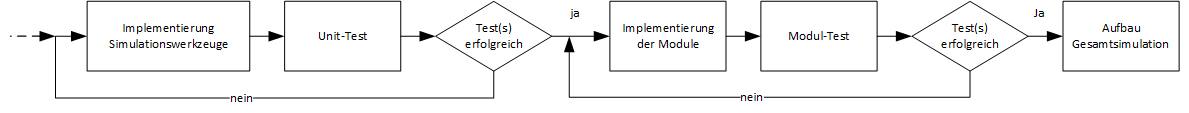
\includegraphics[width=1.0\linewidth]{ImpProzess.PNG}
	\caption{Flussdiagramm des Implementierungs-Prozess}
	\label{fig: ImpProzess}
\end{figure}
\section{Simulationswerkzeuge}
Unter Simulationswerkzeugen sind Funktionen zu verstehen, die in allen Teilen des Simulations-Frameworks vorkommen. Dies umfasst beispielsweise das Einlesen und Schreiben von Simulationsparametern oder mathematische Funktionen wie Integration oder Interpolation. Es ist offensichtlich, dass besagte Funktionen als erstes implementiert werden müssen, damit die Module im späteren Verlauf auf diese zurückgreifen können. Diese Werkzeuge wurden eigens in das Modul \textit{Tools} implementiert. Auch die in \ref{sec:OSBib} beschriebenen Bibliotheken fallen unter diese Werkzeuge. Die implementierten Simulationswerkzeuge werden in Tabelle \ref{tab: SimWerk} zusammengefasst.
\begin{table}[h]
\centering	\begin{tabular}{lp{11cm}}
		\textbf{Funktion/Klasse} & \textbf{Kurzbeschreibung}\\
		 Constants & physikalische Konstanten\\\\
		 DataLogger & Erzeugung von Text-Files (Output der Simulation)\\\\
		 LinearInterpolation & Ein- und zweidimensionale Interpolation \\\\
		 MatFileReader & Funktionen zum Einlesen von .mat-File\\\\
		 ODESolver & Template(s) für numerische Integration\\\\
		 readInData & Funktionen zum Einlesen von Parametern aus Text-Files\\\\
		 Transformation & Matrizen für Koordinatentransformation
	\end{tabular}
\caption{Simulationswerkzeuge der generischen Flugzeugsimulation}
\label{tab: SimWerk}
\end{table}
\newpage
\subsection{Unit-Tests}
Um sicherzustellen, dass die Werkzeuge korrekt implementiert wurden, wurden Unit-Test definiert. Dazu wurde das von Visual Studio bereitgestellte Microsoft-Komponententest-Frameworks für C++ genutzt, um die Tests manuell durchzuführen. Die Unit-Tests wurden in einen gleichnamigen Projektordner ausgelagert. An dieser Stelle werden nicht alle Test erklärt. Vielmehr soll das Test-Schema erläutert werden. In dieser Arbeit wird das AAA-Schema  (Arrange, Act, Assert) nach \cite{Microsoft.2018}  genutzt. Dazu werden die Tests in die zuvor genannten Abschnitte aufgeteilt. Im einzelnen haben die Abschnitte folgende Bedeutung \cite{Microsoft.2018}: 
\begin{itemize}
	\item  \underline{Arrange} dient der Initialisierung des Tests. Die benötigten Objekte werden initalisiert und Parameter für den Testfall festgelegt.   
	
	\item  Innerhalb von \underline{Act} wird die zu testende Methode mit den zuvor definierten Testfall/Parametern aufgerufen.
	
	\item Im Abschnitt \underline{Assert} werden die Referenzwerte mit den Werten aus dem eigentlichen Test vergleichen. Wird eine Übereinstimmung festgestellt, erhählt der Testfall seine Bestätigung durch das Framework.
\end{itemize}
Die Referenzwerte wurden entweder selbst festgelegt (z.B. Einlesen eines Parameters) oder es wurde Matlab genutzt, um Referenzwerte zu generieren (z.B. Interpolation). \\
Nach \cite{TuxFamily.2018} handelt es sich bei \textbf{eigen} um eine vollständig getestete Bibliothek. Aus diesem Grund wurden nur Unit-Tests für einige wichtige Funktionen durchgeführt. Bei der auf \cite{Hulbert.2013} beruhenden MatFileReader-Klasse wird nur der selbst geschrieben Code getestet. Eine Außnahme bei den Unit-Test stellt das Header-File Constants, bei der lediglich physikalische und mathematische Konstanten hinterlegt sind. Die Tests wurden im gleichnamigen Modul implementiert.

\section{Implementierung und Testen der Module}
In Abschnitt \ref{sec:AufbauModule} wurde bereits der Aufbau der Module erläutert und in Tabelle \ref{sec:Ausbaustufen} die für die Simulation benötigten Module aufgelistet. Um deren Funktionalität nachzuweisen, wurden Modul-Tests durchgeführt. Wie schon erwähnt, wird die 6 Dof-Simulation nach \cite{Olucak.15.02.2017} genutzt, um das Simulations-Framework zu testen. Somit liegen nur zu den dort verwendeten Modellen Referenzwerte vor. In diesem Abschnitt beziehen sich die Tests nicht auf das jeweilige Gesamtmodul, sondern lediglich auf die bisher implementierten Klassen.
Die Schwierigkeit, die mit den Modul-Tests einhergeht, ist die Definition der Testfälle. Ziel ist es eine größtmögliche Testabdeckung zu haben, um zu garantieren, dass das Modul wie gewünscht funktioniert. Bei einigen Modulen ist das Testen nur bedingt oder  nur im Gesamtsystem-Test möglich. Dies betrifft beispielsweise das \textit{Autopilot} und \textit{Guidance} Modul. Für beide Module werden Parameter von anderen Modulen benötigt z.B. die Flugzustände. \\Eine weitere Problematik besteht bei den verschiedenen  Modellen der Ausbaustufen.  Für die Simulation mit 3 Freiheitsgraden liegt keine Referenz vor. Ähnlich verhält sich die 6 Dof-Simulation mit Fehlermodellen. Es liegen aktuell keine Modelle für Sensorik und Aktuatorik vor. Somit können an dieser Stelle keine Modul-Tests für die zusätzlichen Module erfolgen.
In Tabelle \ref{tab:modultests} werden die Module  und deren Testfälle aufgezeigt, für die ein Modul-Test in Betracht kommt.\\
\begin{table}[h]
\centering	\begin{tabular}{l p{12cm}}
		\textbf{Modul} & \textbf{Beschreibung Testfall}\\
		Atmosphere & Bei dem hier hinterlegten Modell  handelt es sich um die US Standard-Atmosphäre von 1976.  Temperatur, Druck, Dichte und Schallgeschwindigkeit sind hierbei abhängig von der Flughöhe. Somit werden die zuvor beschriebenen Größen von 0-10000m berechnet und mit Daten der Standard-Atmosphäre verglichen.\\\\
		Aerodynamic & Hier wird ein Windtunnel bei konstanter Höhe simuliert. Es werden Machzahl, Anstellwinkel und Höhenruder-Winkel variiert. Es ist ersichtlich, dass nur die Längsbewegung betrachtet wird. Dies ist auf mangelnde Referenzwerte für die Seitenbewegung zurückzuführen. Ziel dieses Tests ist es die Polare des Flugzeuges abzufahren und mit den Matlab-Daten zu vergleichen. \\\\
		Guidance &  Es wird lediglich getestet, dass für den jeweiligen Zeitschritt die richtige Soll-Querbeschleunigung und Trajektorie vorliegt. Das Modul selbst kann erst im Gesamtsystemtest vollständig getestet werden, da die jeweiligen Flugzustände benötigt werden.\\\\
		Trajectory & Der Trajectory-Modul Test testet die korrekte Berechnung der Flugbahn. Hier wird die Matlab-Simulation simuliert. 
	\end{tabular}
\caption{Auflistung der Modultests}
\label{tab:modultests}
\end{table}
\newpage
Aufgrund der Einfachheit des aktuell hinterlegten Schub-Models (Engine-Modul) wurde auf einen Modul-Test verzichtet und der Nachweis über Code-Reading durchgeführt.
Es ist offensichtlich, dass das Trajektorien-Modul erst aufgebaut werden konnte, nachdem die dafür benötigten Module bereits erfolgreich getestet wurden. Wie auch bei den Unit-Tests wurden die Modul-Tests in einem eigenen Modul implementiert. Die Überprüfung der Tests erfolgte rein qualitativ und die Ergebnisse  wurden im Ordner \textbf{Test Results} hinterlegt. Dies dient als Referenz für zukünftige Änderungen. 


\section{Validierung des Simulations-Framework}
Abschluss des Implementierung stellt der Gesamtsystemtest des Simulations-Framework. Dazu wird das \textbf{Aircraft} Modul mit den Simulationsparametern nach \cite{Olucak.15.02.2017} initialisiert.\\
Ziel von \cite{Olucak.15.02.2017} war es, den Flugzustandsregler zu testen. Dem Vorgaberegler wurden Querbeschleunigungen für jeden Zeitschritt als Soll-Wert vorgegeben. Ziel war es, dass das Flugzeug den Querbeschleunigungen folgt.\\ In Abbildung \ref{fig:valSim} sieht man, wie der Ist-Wert des Reglers den Soll-Werten der Guidance  sehr gut folgt. Die anfänglichen Schwingungen sind auf die Initialisierung der Simulation am Trimmpunkt zurückzuführen. Da die Arbeitspunkte durch Linearisierung gefunden werden, entsteht ein Modellfehler.
\begin{figure}[h]
	\centering
	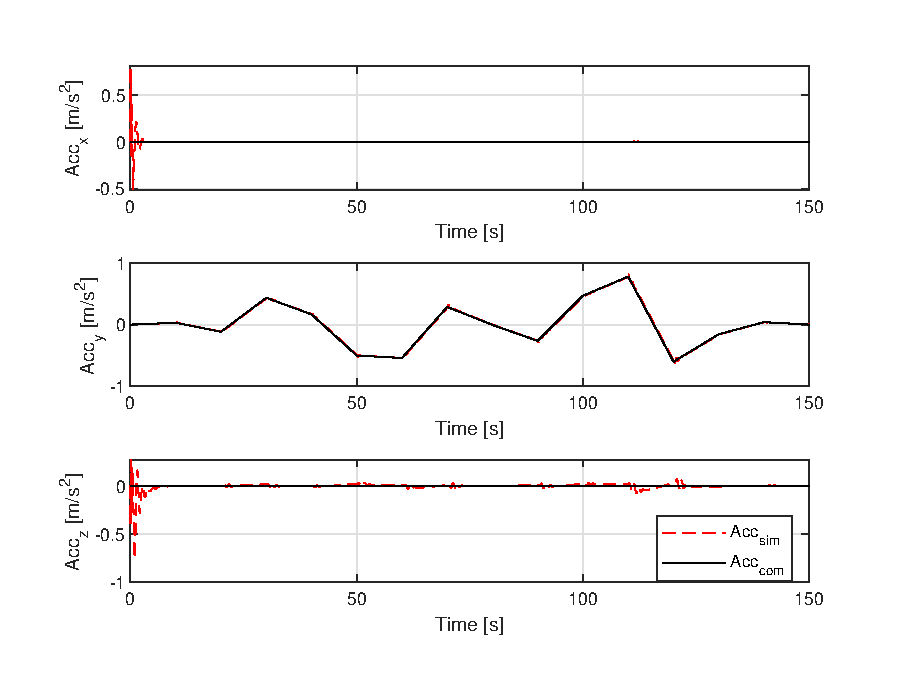
\includegraphics[width=0.7\linewidth]{querbeschleunigungen}
	\caption{Validierung der Simulation}
	\label{fig:valSim}
\end{figure}\noindent\\
Da kein Bahnregler implementiert wurde, ist es weniger zielführend die Trajektorie selbst zu betrachten, da das Flugzeug lediglich den Querbeschleunigungen folgt. Weitere Simulationsergebnisse sind im Anhang unter \ref{sec:simerg} dargestellt. \newpage
Nachfolgend werden die Ergebnisse von Matlab und C++ verglichen.

 \begin{minipage}{0.49\linewidth} 	
 		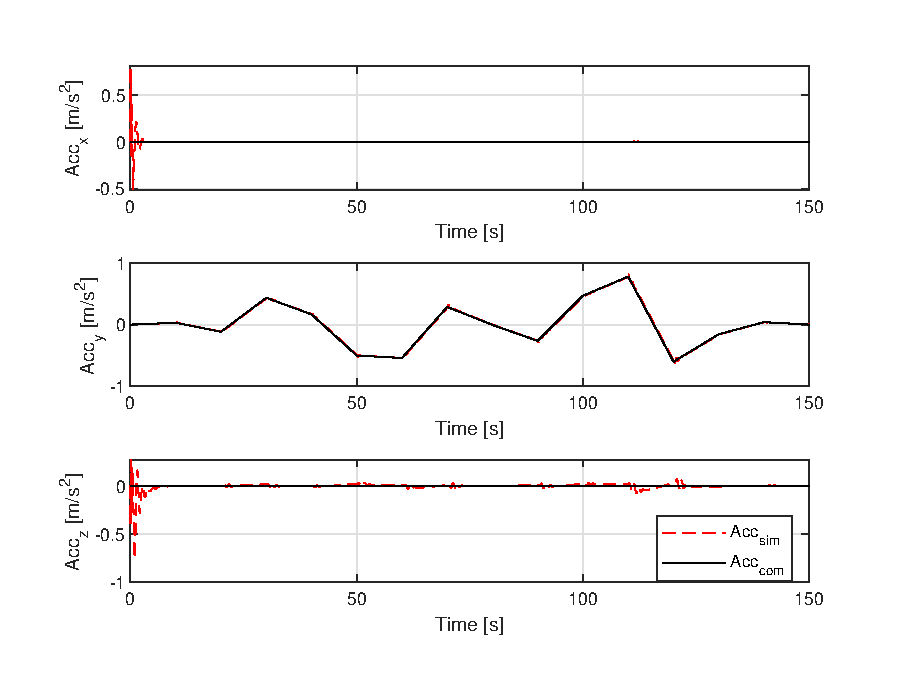
\includegraphics[width=1.0\linewidth]{querbeschleunigungen}
 \end{minipage}
 \begin{minipage}{0.01\linewidth}
	\hfill
\end{minipage}
 \begin{minipage}{0.49\linewidth}
		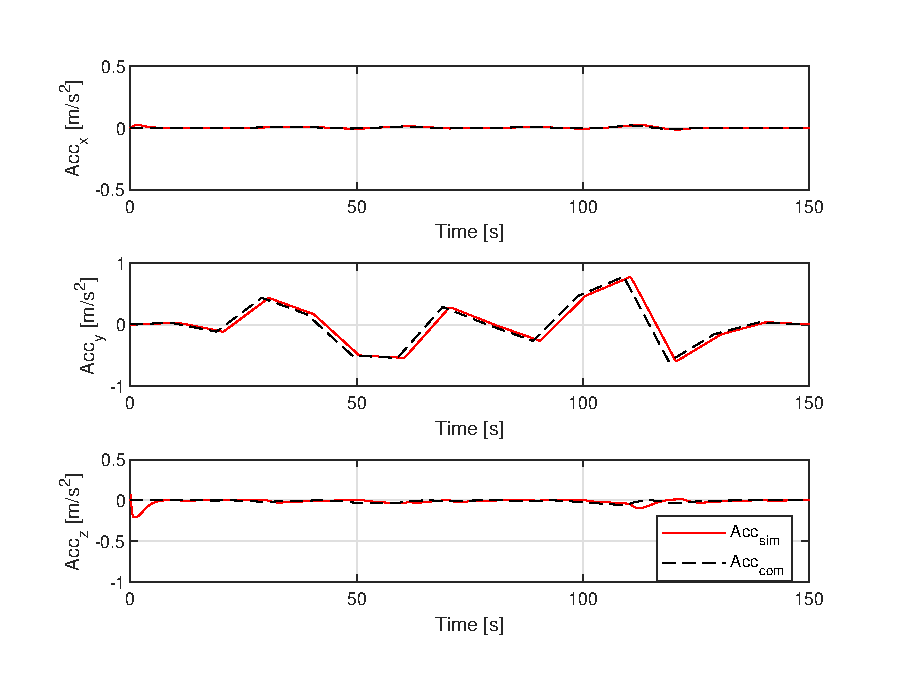
\includegraphics[width=1.0\linewidth]{matSim}
\end{minipage}
\captionof{figure}{Vergleich der Simulationsergebnisse, links C++, rechts Matlab}\noindent\\
Bei beiden Simulationen sind die Initialisierungsfehler zu erkennen, wobei in C++ die anfänglichen Schwingungen größere Amplituden besitzen. Offensichtlich folgt die Simulation in C++ der Soll-Werten besser als in Matlab. Zudem sind auch numerische Unterschiede zu erkennen. In \cite{Unbekannt.2012} und \cite{Unbekannt.2011} wurden diese numerischen Unterschied zwischen Matlab und C/C++ diskutiert. Beruhend auf diesen Quellen ist es zu erwarten, dass die beiden Ergebnisse nicht vollständig übereinstimmen und die Berechnung in C++ genauer ist. Die Simulation nach \cite{Olucak.15.02.2017} diente nur der Validierung und nicht der Verifikation. Das Ziel, dass das Flugzeug den Querbeschleunigungsvorgaben folgt, wurde erfüllt. Die Ausbaustufe mit 6 Freiheitsgraden konnte somit validiert werden.\\ Die höchste Ausbaustufe liefert die gleichen Ergebnisse wie die Ausbaustufe ohne Fehlermodelle. Wie in Abschnitt \ref{sec:Ausbaustufen} beschrieben, sind nur Methoden implementiert, die ein fehlerfreies Verhalten simulieren. Somit konnte auch diese Ausbaustufe erfolgreich getestet werden. Auf eine Visualisierung wurde an dieser Stelle verzichtet.
\newpage
\subsection{Direktvergleich Rechenzeit Matlab und C++}
In Abbildung \ref{fig:direktvergleich} wird die Rechenzeit der Simulation in Matlab und C++ gegenübergestellt. Der Performance Gewinn in C++ ist offensichtlich zu erkennen.
\begin{figure}[h]
	\centering
	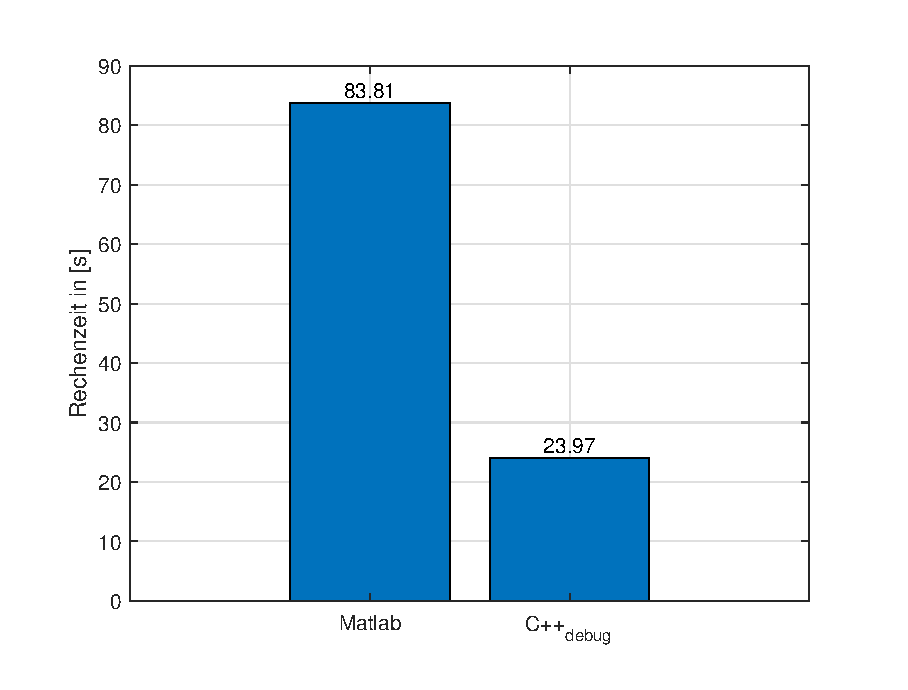
\includegraphics[width=0.6\linewidth]{Direktvergleich}
	\caption{Direktvergleich Matlab und C++}
	\label{fig:direktvergleich}
\end{figure}\noindent \\
Betrachtet man das Ergebnis von der quantitativen Seite und berechnet den relativen Rechenzeitunterschied ist das C++ Programm 71,4\% schneller als Matlab. Dieses Ergebnis ist weniger verwunderlich, da C++ das Programm in Maschinencode übersetzt. Matlab ist eine proprietäre Programmiersprache die auf dem jeweiligen Rechner interpretiert wird und kann dementsprechend die Ressourcen des Computers nicht voll ausnutzen.\\
Mit diesem Ergebnis wurde ein Ziel dieser Arbeit, die Rechenzeit zu reduzieren, erreicht.
